\documentclass[final, fmstyle, lic]{tesis}

% paquetes usados
%\usepackage[chapter, spanish]{theorems}
\newtheorem{theorem}{Teorema}[chapter]
\newtheorem{lemma}{Lema}[chapter]
\newtheorem{proposition}{Proposición}[chapter]
\newtheorem{corollary}{Corolario}[chapter]
\newtheorem{definition}{Definición}[chapter]
\newtheorem{example}{Ejemplo}[chapter]
\newtheorem{observation}{Observación}[chapter]

\usepackage{symbols}
\usepackage{graphicx} %usar imágenes externas
\usepackage{url}
\usepackage{blindtext}
\usepackage[table,xcdraw]{xcolor}

% Agregado por mi Saul para tener tablas que puedan usar varias paginas
\usepackage{longtable}
% Agregado por mi Saul para algunas citas directas
\usepackage{csquotes}
\usepackage{wrapfig}
\usepackage{float}

\usepackage{caption}
\usepackage{subcaption}

\usepackage[utf8]{inputenc}  % descomentar para teclado en español de Unix, Mac y posiblemente Windows
\usepackage[T1]{fontenc} % this helps hyphenate Spanish vocabulary with acute accent 
%\usepackage[latin1]{inputenc}  % descomentar para teclado en español de Unix y posiblemente también de Windows
%\usepackage[applemac]{inputenc}  % descomentar para teclado en español de Mac
\usepackage[spanish]{babel}
\decimalpoint

\setlength{\parskip}{2mm}	%Espaciado entre párrafos 

\graphicspath{ {./images/} } %Carpeta que contiene imagenes del documento

\usepackage{hyperref}
%\usepackage{urm}
% datos de la tesis
\title{Desarrollo de un videojuego multijugador para la enseñanza de la programación de computadoras}
\author{150424}{Saúl Núñez Castruita}
\authorb{}{}
\director{M.A.T.I}{Abraham López Nájera}
\directorb{Dr.}{Luis Carlos Méndez González}
\directorbp{«Profesor-Investigador IIT»}  % Dejar en campo en blanco si no hay segundo asesor
\sinodala{Dr.}{Nombre del Sinodal A}
\sinodalb{Dr.}{Nombre del Sinodal B}
\sinodalc{Dr.}{Nombre del Sinodal C}
\titular{Dr.}{Francisco Lopez Orozco} % Titular de Seminario de Titulación II

% comenta para automático:
\termyear{\today}

\begin{document}
\pagenumbering{roman}

\maketitle     % esto hace las portadas
\approvalpage  % esto hace la pagina de aprobaci√õn
\approvalprint  % esto hace la pagina de aprobaci√õn
%\approvalprint % esto hace la pagina de aprobaci√õn de impresión. Comentar si sólo un alumno
\originalpage

% Inicio de los Agradecimientos
\begin{thanks}

%[Sustituye este texto escribiendo tus agradecimientos.
%La sección de agradecimientos reconoce la ayuda de personas e instituciones que aportaron significativamente al desarrollo de la investigación. No te debes exceder en los agradecimientos; agradece sólo las contribuciones realmente importantes, las menos importantes pueden agradecerse personalmente. El nombre de la agencia que financió la investigación y el número de la subvención deben incluirse en esta sección. Generalmente no se agradecen las contribuciones que son parte de una labor rutinaria o que se reciben a cambio de pago. 

%Las contribuciones siguientes ameritan un agradecimiento pero no justifican la coautoría del artículo: ayuda técnica de laboratorio, préstamo de literatura y equipo, compañía y ayuda durante viajes al campo, asistencia con la preparación de tablas e ilustraciones o figuras, sugerencias para el desarrollo de la investigación, ideas para explicar los resultados, revisión del manuscrito y apoyo económico”.]

Quiero darle las gracias a mis asesores por las sugerencias de cómo mejorar este trabajo. 

También agradezco a los diferentes docentes que me dieron parte de su día para revisar el producto aquí creado a fin de ver que cumpliera los requisitos el producto creado y por sus recomendaciones para mejorarlo, algunas de las cuales se pudieron aplicar. 

Así como los diferentes profesores del Seminario de Titulación por su apoyo para que este documento tenga el menor numero de errores ortográficos y problemas de dicción en sus enunciados.

\end{thanks}
% Fin de los Agradecimientos
\setcounter{page}{6}
% Inicio de Dedicatoria

\chapter*{Dedicatoria}


[Aquí escribe tu dedicatoria.]


% Fin de Dedicatoria

% los siguientes comandos producen Ìndices.
% tablas y figuras en el documento de la tesis
\tableofcontents
\listoffigures
\listoftables

% Inicio de Resumen
\chapter*{Resumen}
\markboth{chapter name}{Sinopsis}


[Sustituye este texto escribiendo tu sinopsis o resumen. Es un panorama general de todo lo que el lector encontrará en tu documento, en no más de una página. Recuerda que este, junto con el título, son la parte más leída de tu documento cuando alguien más lo busca en las bases de datos, el “punto de venta''.]


% Fin del Resumen

\setcounter{page}{1}

\setcounter{page}{1}
\pagenumbering{arabic}
% Inicio de \section*{Introducción}\label{introduccion}
\chapter*{Introducción}\label{introduccion}

[Redacte de manera coherente en una cuartilla cuál es la nueva contribución, su importancia y por qué es adecuado para sistemas computacionales. Se sugiere para su redacción seguir los cinco pasos siguientes: 1) Establezca el campo de investigación al que pertenece el proyecto, 2) describa los aspectos del problema que ya han sido estudiado por otros investigadores, 3) explique el área de oportunidad que pretende cubrir el proyecto propuesto, 4) describa el producto obtenido y 5) proporcione el valor positivo de proyecto.]


\chapter{Planteamiento del Problema}
En este capítulo se entrara en detalle sobre los términos relacionados al proyecto y analizamos 
trabajos anteriores sobre software enfocados en la enseñanza de programación de computadoras desde los 
60s hasta la actualidad. De igual manera, se define que atacaremos con este proyecto, una problemática y que objetivos tiene el proyecto.

\section{Antecedentes}

\subsubsection{Videojuegos como método de enseñanza}
El área de serious games puede pensarse como dos grandes áreas: entre ellas existe el edutainment, 
aplicaciones informáticas con animaciones, elementos multimedia que muestran la información de una manera divertida; 
y los videojuegos, creados con la pretensión explicita de enseñar, incluyen el entrenamiento a base de simuladores, 
la transmisión de la información o incluso, la promoción de alguna idea o marca [1]. 
La principal diferencia para es la difusión del contenido, el edutainment prioriza 
la difusión del contenido de manera lúdica, mientras que los videojuegos para enseñar deciden 
sacrificar la parte lúdica para explorar de mejor manera los conocimientos y lo hace de maneras más complejas [1].
Mucho desarrollo en el área y uno de los primeros en adoptar los serious games fue la milicia, 
se usan para el adiestramiento militar, sin contar con el número de simulaciones de distintos vehículos militares [1]. 
Asimismo, han existido serious games de política, con diferentes propósitos, como la comunicación de ideas, 
criticar a oponentes o reproducir sus discursos, 
algunos ejemplos son los news games que mezclan lo periodístico con la denuncia política y exponen una problemática de un determinado lugar y tiempo. 
Adicionalmente existen géneros como los advergames, usados para publicidad, 
los de salud que permiten a los estudiantes aprender sin temor a equivocarse con un ser humano, 
los videojuegos artísticos y los videojuegos religiosos [1].

\subsubsection{Evolución de la enseñanza de la programación}
Podemos notar como punto importante la creación de Pascal a finales de los 60s y principios de los 70s por parte de Niklaus Wirth, un lenguaje enfocado en la enseñanza de técnicas de programación, con una nueva metodología de programación denominada programación estructurada [2]. Sin embargo, no todo es tan claro, no ha existido un consenso de los métodos a utilizar y no ha existido alguno que se haya impuesto. 
Existen métodos para la enseñanza de otros paradigmas de programación como el funcional, el imperativo o el imperativo orientado a objetos; y dentro de estas divisiones hay quienes enseñan a programar mediante un lenguaje particular o quienes emplean un lenguaje algorítmico que pudiera adaptarse a otros lenguajes de programación [2].
Sin embargo, podemos destacar la existencia de algunas nuevas herramientas:

\subsubsection{LOGO}
Logo es un lenguaje de programación diseñado como una herramienta para aprender programación. 
Permite mover una tortuga (originalmente una creatura robótica) a cualquier dirección 
mediante introducir comandos a la computadora [3] cómo se nota en la \ref{fig:logo_scrn}.

\begin{figure}[h]
    \caption{LOGO}
    \centering
    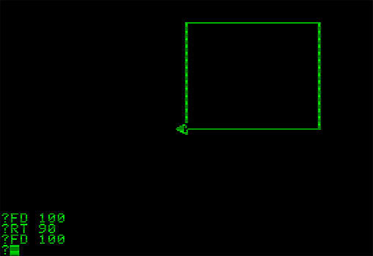
\includegraphics[width=0.5\textwidth]{logo}
    \label{fig:logo_scrn}
\end{figure}

\subsubsection{Pascal}
Lenguaje creado en 1970 por Niklaus Wirth para enseñar programación estructurada, 
paradigma de programación donde se pone énfasis en las 
estructuras condicionales y cíclicas, sin GOTO [4]. 
Fue comúnmente usado durante después de la primera mitad de los 70s y los 80s 
debido a que estaba disponible en un gran número de computadoras, 
así como por su claridad y seguridad, no era raro que fuera usado para la 
producción de software.

\subsubsection{Python}
Diseñado por Guido Van Rossum originalmente estaba pensado 
para como un lenguaje de scripting para el sistema operativo Amoeba [5]. 
Su ventaja en el ámbito educativo es su facilidad de uso, comúnmente descrito 
como poder programar en inglés y la gran cantidad de librerías que permiten 
crear cosas complejas de manera rápida.

\subsubsection{Lego WeDo 2.0}
Es un kit diseñado para introducir a niños y niñas a la robótica, 
construyen pequeños robots con LEGO y de diferentes 
formas pueden programarlos para que se muevan. 
Normalmente hacen uso de programación por bloques.

\subsection{Trabajos relacionados}
En la actualidad, muchos programas para enseñar programación utilizan 
drag-and-drop para realizar la tarea de programación, 
a esta se le conoce como block-based programming [6]. 
Ejemplos de herramientas de esta categoría incluyen el entorno Scratch, 
que permite crear pequeños juegos o animaciones con sus herramientas, 
como se nota en la \ref{fig:scratch_scrn} y Code.org, donde hay diversas actividades 
para aprender a programar.

\begin{figure}
    \caption{El entorno de programación Scratch}
    \centering
    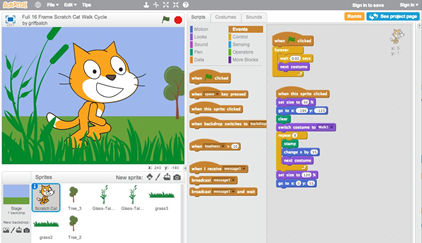
\includegraphics[width=0.5\textwidth]{scratch}
    \label{fig:scratch_scrn}
\end{figure}

Similar, aunque a diferencia de este proyecto, Lego WeDo va orientado a la robótica. Según la clase, eligen de una de las diferentes opciones disponibles para construir y los alumnos siguen unas instrucciones similares a otros kits de LEGO, y puede ser programado en Scratch o en un software propio de LEGO [7]. Incluye un hub con conectividad bluetooth, donde se pueden conectar sensores y motores [8], como se puede ver en la \ref{fig:wedo}. El software de LEGO es igual, block-based programming e incluye sesiones donde los estudiantes aprenden de diversos temas y realizan actividades de programación relacionadas a estos. A diferencia de estos dos, en lugar de ser el profesor la principal fuerza para poner nuevos retos y enseñar nuevos conceptos, acudiremos a mecánicas vistas en videojuegos.

\begin{figure}
    \caption{El entorno de programación Scratch}
    \centering
    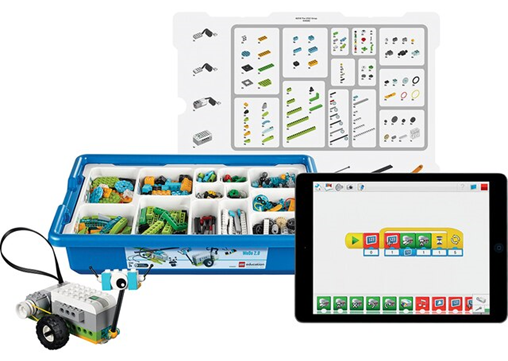
\includegraphics[width=0.5\textwidth]{wedo}
    \label{fig:wedo}
\end{figure}

Por otro lado esta “Kahoot”!, que es una plataforma de game-based learning [9], esta permite a profesores poner quizzes, de los cuales los estudiantes eligen la respuesta en sus teléfonos y en una pantalla más grande a la que tiene acceso el profesor se muestra la pregunta actual con sus posibles respuestas, así como la posición en la que están los alumnos entre cada pregunta, como se nota en la \ref{fig:kahoot}. Este proyecto es útil para las evaluaciones, sin embargo, de manera similar a este el profesor tiene el control del tema a trabajar y lo controla desde un lobby. 

\begin{figure}
    \caption{Kahoot!}
    \centering
    \label{fig:kahoot}
\end{figure}

Hay una variedad de juegos de programación, como CodingGame, que es un sitio de minijuegos donde se ofrecen instrucciones sobre el punto del juego y cuenta con un IDE para programar una solución para pasarlo. Asimismo, CodeCombat, un juego de dungeon crawling donde se debe programar para avanzar en el juego [10], hay aspecto multijugador y al igual a “Kahoot!” uno puede ser parte de un lobby de una clase y el profesor puede ver el avance de sus alumnos, pero cada jugador avanza a su ritmo. Similarmente, en Screeps un MMO de estrategia para programadores de Javascript y CheckIO, se deben resolver problemas en Python [11]. Sin embargo, todos están enfocados además en la enseñanza de un lenguaje de programación (Python o Javascript son opciones comunes), por lo que para un principiante puede ser un punto de contención adicional el aprender la sintaxis durante la práctica. Similarmente, en el área de edutainment existen juegos como Human Resource Machine, Hack ‘n’ Slash, TIS-100, donde a excepción del ultimo están enfocados a desarrollar una lógica para programar, TIS-100 agrega un lenguaje ensamblador con programación a base de “nodos”, cada nodo solo acepta programas pequeños, se comunican varios nodos para crear programas más complejos, TIS-100 es más apto para enseñar sistemas distribuidos en lugar de programación básica.

\section{Definición del problema}
La enseñanza de programación es regularmente una dualidad con la enseñanza de un lenguaje de programación, donde se enfoca en la enseñanza de la sintaxis y en la enseñanza y práctica de hilar la lógica necesaria para crear un programa para computadoras, donde entran técnicas como [12]:
\begin{itemize}
    \item Descomposición de problemas complejos
    \item Reconocimiento de patrones para buscar similitudes entre problemas
    \item Abstracciones
    \item Algoritmos
\end{itemize}}

La enseñanza de programación es un proceso complejo, donde el alumno tiene que acostumbrarse a razonar la forma de solucionar un problema (a base de descomposición) y aprender un lenguaje de programación con todas las idiosincrasias que este tenga, desarrollando los debidos modelos mentales sobre el funcionamiento del lenguaje y sobre la notación para resolver un problema [13]. La sintaxis de un lenguaje de programación puede ser complicado para un principiante, se ha encontrado que estos tienen dificultad para encontrar errores gramaticales en su código [13]. Para esto, sería mejor dotar a alguien aprendiendo a programar con la habilidad de razonar problemas en un entorno donde no tengan que razonar mucho la sintaxis del lenguaje, y haya aspectos visuales que permitan al usuario experimentar programando y desarrollar los modelos mentales, pero reduzcan la carga cognitiva de usar una herramienta como un lenguaje de programación escrito por texto. 


\section{objetivo general}
Desarrollar un videojuego multijugador colaborativo que permita a alumnos aprender programación estructurada usando un lenguaje de programación visual. 

\subsection{Objetivos específicos}

\begin{enumerate}
    \item Creación de un documento de diseño.
    \begin{enumerate}
        \item Diseño de puzzles en un entorno colaborativo relacionados a distintos conceptos de la programación estructurada. 
        \item 	Crear un mundo virtual que conecte los diversos puzles para enseñar a los alumnos programación 
    \end{enumerate}
    \item Crear un entorno de programación por bloques para que los alumnos puedan programar soluciones de puzzles.
    \item Desarrollar un componente de servidor para la creación de lobbies.
    \item Desarrollar el software en Javascript para el navegador web.
    \item Validar resultados a través de pruebas estadísticas.
\end{enumerate}

\section{Pregunta de Investigación}
¿Qué ventajas existen en la enseñanza de programación mediante el videojuego propuesto?

\section{justificación}
Un videojuego colaborativo permitiría tener ventajas como el desarrollo de las habilidades cognitivas, sociales en un ambiente de colaboración permite a sus integrantes encontrar nuevas formas de atacar problemas, algunas de estas de especial importancia para la programación. 
Adicionalmente, los videojuegos son peculiarmente efectivos para la resolución de problemas, debido a que permiten “aprender haciendo” donde el proceso de aprendizaje es una constante practica e interacción con tareas más complejas donde los jugadores encuentran reglas subyacentes que son de utilidad para resolver los problemas que nos plantee el juego [14]. Peculiarmente, este método de aprendizaje iterativo es muy cercana a la manera en la que resolvemos problemas en la vida diaria, en esta regularmente resolvemos problemas por analogía, donde recurrimos a esquemas (paquetes de información sobre las propiedades del problema como: el conocimiento antes de intentar resolver el problema, a que se quiere llegar, los posibles pasos y aquello que es permitido y las consecuencias de escoger incorrectamente) y se recupera el marco que se creó anteriormente para resolver este nuevo problema [14].
Un videojuego para la enseñanza de programación con los puntos anteriores, puede ser una excelente herramienta para la enseñanza en salones de clase de los elementos básicos de la programación y permitir a principiantes desarrollar la habilidad de resolver problemas. Adicionalmente, un videojuego corto puede ser una excelente herramienta para una clase de Hour of Code (una propuesta para en una hora, introducir a pequeños o a grandes a la computación o a la programación).


\subsection{Alcances y limitaciones}
\chapter{Marco teórico}
En esta sección entramos en detalle el marco conceptual y el marco tecnológico. En la primera sección se verá la forma de aprovechar los videojuegos para la enseñanza, sus ventajas y la forma de enseñanza que comúnmente aprovechamos con estos, además tocamos temas relacionados a la programación por bloques y la metodología de software a usar y sus artefactos. En la segunda sección discutimos de tecnologías aptas para la realización del proyecto.

\subsection{Marco Conceptual}
\subsubsection{Game-based learning y educación colaborativa}
Game-based learning es “en formación en la cual los contenidos teóricos son presentados por medio de un videojuego” [15] y contienen elementos como [16]:
\begin{itemize}
    \item Historia para darle inmersión a los jugadores
    \item Gamificación, como rankings o un sistema de puntos
    \item Feedback inmediato, algunos juegos tienen información como en que se equivocaron y una oportunidad de realizarlo otra vez
    \item Simulación de una situación de la vida real, permitiendo la práctica segura en ambientes cercanos a donde aplicarán su conocimiento
\end{itemize}

Los videojuegos pueden ser una muy poderosa herramienta para el aprendizaje: permiten el aprendizaje \textit{Just In Time} que bajo desafíos realizables empujan al 
jugador a ser competente y nos ayudan a fomentar el pensamiento crítico [17]. 
El aprendizaje \textit{Just In Time} ofrece el conocimiento necesario para hacer una tarea justo cuando es necesario [18]. 
Hay métodos en los que la enseñanza \textit{JIT} ocurre naturalmente como ver un video de \textit{Youtube} cuando no sabemos cómo realizar una tarea, 
en los videojuegos es natural cuando hay introducciones a acciones en el juego como la forma en la que lo invocamos o las acciones que realizan, 
ya sea mostrando una interfaz gráfica con la forma de invocarlo.
Se encontró que los estudiantes en el aprendizaje colaborativo los alumnos se enseñan uno al otro al responder a dudas y 
clarificar preconcepciones, desarrollan comunicación oral y capacidad de liderazgo, aumenta la retención del material, 
la responsabilidad y expone a los alumnos a perspectivas diversas [19].
Se ha encontrado que los videojuegos colaborativos agregan ventajas como el trabajo en equipo, el pensamiento creativo, 
la comunicación y la colaboración [20].

\subsubsection{Block-based programming}
Block-based programming se ha establecido como la forma de introducir a aquellos que quieren aprender a 
programar seguido por el éxito de Scratch y Code.org [6]. 
Este método de programación usa piezas de un rompecabezas como metáfora para proveer al usuario pistas sobre cuales instrucciones son válidas [6]. 

\subsubsection{Kanban}
Kanban es una metodología ágil para el desarrollo de software con un énfasis 
en la entrega continúa teniendo en cuenta la capacidad del equipo [21]. 
Las métricas de Kanban son las siguientes [22]:
\begin{itemize}
    \item \textbf{Diagrama de flujo acumulativo \ref{fig:flujo_acumulativo}:} Provee información relacionada con la capacidad del equipo. Está basado en tiempo y muestra cómo se mueven las tarjetas de izquierda a derecha en el tablero. La altura de las bandas muestra el número de tarjetas en esa etapa durante cierta unidad de tiempo.
    \begin{figure}[h]
        \caption{Diagrama de flujo acumulativo}
        \centering
        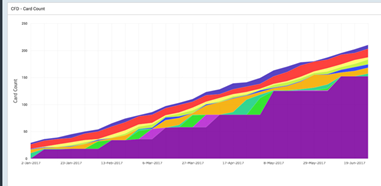
\includegraphics[width=0.5\textwidth]{flujo_acumulativo.png}
        \label{fig:flujo_acumulativo}
    \end{figure}
    \item \textbf{Gráfica de distribución de tiempos de ciclo \ref{fig:distribucion_tiempos_ciclos}:} Es útil para ver la frecuencia con la que las tarjetas son completadas a lo largo del tiempo.
    \begin{figure}[h]
        \caption{Gráfica de distribución de tiempos de ciclo}
        \centering
        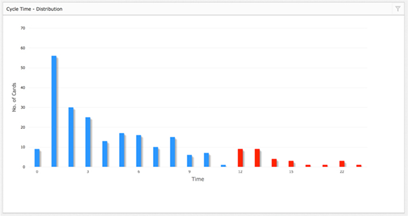
\includegraphics{distribucion_tiempos_ciclos}
    \end{figure}
\end{itemize}

\subsection{Marco tecnológico}
Para el desarrollo de este proyecto es necesario tener herramientas para las partidas con otros usuarios, así como manera de usar librerías probadas y comúnmente usadas.

\subsubsection{Unity3D}
Es un motor que permite diseñar videojuegos. Permite usar C# para programar el juego, compilando, usando Mono. [23] Es un motor muy capaz que permite desarrollar videojuegos 2D y 3D, con una variedad de herramientas para facilitar el desarrollo.
Unity puede crear el juego para varios entornos, como consolas de videojuegos como la Nintento Switch, el Xbox One, PS4, Windows, MacOS, Linux, Android, iOS, o la web mediante WebGL [24]. La ventaja del entorno web es la posibilidad de conectar Unity con la pagina web que lo alberga, con esto puede puedo interactuar con elementos HTML o con librerías JS, en este caso lo conectaremos con Blocky.
\begin{figure}
    \caption{Algunas capacidades de Unity para el desarrollo de videojuegos: animaciones, máquina de estados y para videojuegos 2D, un editor de sprites}
    \centering
    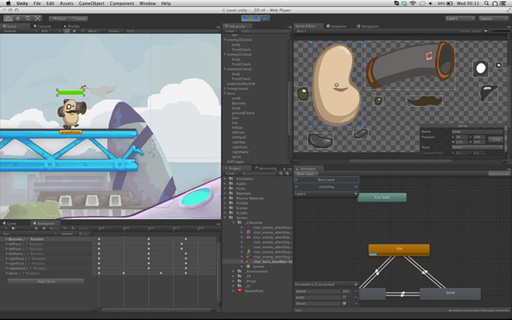
\includegraphics{unity}
\end{figure}

\subsubsection{Blocky}
Librería de Google que permite al usuario escribir código usando bloques como se nota en la \ref{fig:blocky_example} y compila el resultado a diferentes lenguajes entre ellos Javascript, Dart, Python, Lua y PHP.

\begin{figure}
    \caption{Un ejemplo de un juego usando la librería de Blocky}
    \centering
    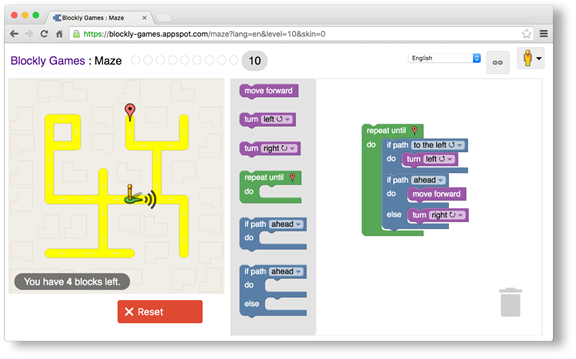
\includegraphics{blocky_example}
    \label{fig:blocky_example}
\end{figure}

\subsubsection{ASP .NET Core}
Framework para sitios web de Microsoft. [25] Será usado como la base para hospedar la API del servidor, servir los archivos del juego, así como páginas de landing y de creación de lobbies.

\subsubsection{SignalR}
Es una librería de Microsoft que nos permite hacer comunicación en tiempo real web. Permite ser usado para crear RPC, o llamadas de procedimiento remoto. [26] Su principal ventaja es que mandar mensajes al servidor es muy fácil a otras soluciones, hay una API definida que la librería se encarga que de que en cada request sea cumplida el schema de la API y se encarga de la serialización y deserialización de cada comunicación. Así como pasar información de cambios al cliente ocurre de manera rápida, maneja el protocolo de transferencia y evita mucha configuración que de otra forma seria necesario.

\subsubsection{Git}
Git es el sistema de control de versiones más popular del mundo, fue creado en 2005 por Linus Torvalds [27]. Es un ejemplo de un DVCS, un sistema distribuido de control de versiones, a diferencia de sistemas donde en un solo lugar esta todo el historial de versiones como CVS o Subversion, en Git todas las copias funcionales de código son un repositorio que contiene todo el historial de versiones.
En comparación con otros sistemas, Git está diseñado para que la creación de ramas y tags sean operaciones baratas, por lo tanto, rápidas.

Github es un servicio de hospedaje de repositorios Git [28]. Se usara como \textit{repositorio remoto} para sincronizar cambios, además de aprovechar sus funciones para crear pipelines para el continous deployment.
\chapter{Desarrollo del Proyecto}
[Este capítulo se considera el más importante al elaborar el proyecto de titulación. Se describe el procedimiento seguido para lograr el objetivo planteado. Se explica qué y cómo se hizo, además se debe de convencer de que los métodos o procedimientos usados fueron los más adecuados.

Deben detallarse los procedimientos, técnicas, métodos, metodologías y demás estrategias metodológicas requeridas para el proyecto. 
]

\section{Producto propuesto}

\section{Fases (Metodología)}



...
\section{Avances}



\chapter{Resultados y Discusiones}
El siguiente capitulo se trabajó a base de la forma de validación detallada en el capítulo anterior. Y se detallan los resultados obtenidos.

\section{Detalles de resultados}
Se hizo reuniones con profesores de la materia de Fundamentos de Programación, en estas se revisaron los \textit{puzzles} del juego, se les mostró las mecánicas del juego y se revisó con ellos la forma de instalación para ver complejidad. Dado que por falta de tiempo la instalación se hace por el docente en su propia máquina. Las reuniones se realizaron para ver las opiniones del producto realizado para usuarios finales potenciales. Los usuarios a los que tiene más potencial de afectar el juego son a los estudiantes, pero como los profesores son los que implementan el juego en su clase, es importante de primera mano conocer sus perspectivas respecto al juego creado.

Se realizaron cinco reuniones con distintos docentes del departamento de ingeniería eléctrica y computación de la Universidad Autónoma de Ciudad Juárez que imparten o impartieron en los últimos semestres la materia de Fundamentos de Programación en el campus de Ciudad Universitaria.

\subsection{Primera reunión}
Se realizó esta reunión el 6 de octubre del 2021. En esta se revisó el material del juego, se vio el valor didáctico de los diferentes puzzles del juego, y de manera menos detallada, la instalación y el \textit{gameplay}. En la revisión del juego, comento de manera positiva la variedad de los puzzles. Sin embargo, mencionó que debido al diseño de los puzzles que algunos tienen código similar a \textit{C} (figura~\ref{fig:for_puzzle_fail_c}), otro muy parecido a \textit{Python} (figura~\ref{fig:for_puzzle_fail_python}) y algunos adicionales de pseudocódigo, seria complicado para el docente usar este juego para la impartición de su clase porque ``rompería'' con lo visto en clase en algunos temas. Si el profesor tiene que explicar al estudiante que ciertos \textit{puzzles} funcionan de manera diferente a como se explicó en clase, el juego pierda valor didáctico y en el peor de los casos, podría confundir a los estudiantes.
\begin{figure}
    \centering
    \begin{subfigure}{0.4\textwidth}
         \centering
         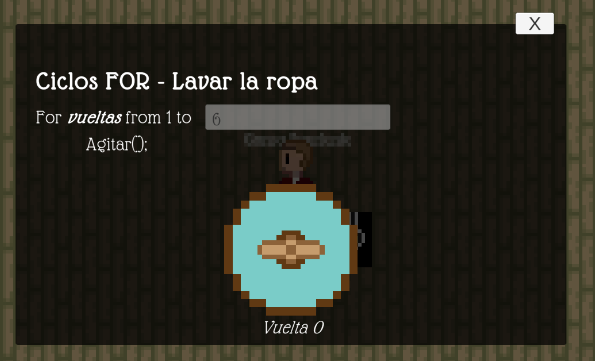
\includegraphics[width=\textwidth]{for_puzzle_fail_python}
         \caption{Este \textit{puzzle} tenía una sintaxis inspirada en \textit{Python} y su uso de \textit{ranges}}
         \label{fig:for_puzzle_fail_python}
     \end{subfigure}
         \begin{subfigure}{0.4\textwidth}
         \centering
         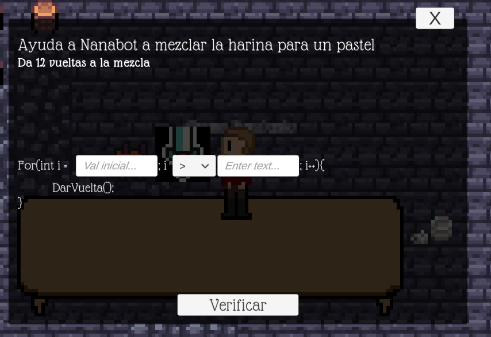
\includegraphics[width=\textwidth]{for_puzzle_fail_c}
         \caption{La sintaxis de este \textit{puzzle} era similar a C}
         \label{fig:for_puzzle_fail_c}
     \end{subfigure}
\end{figure}

Ante estos resultados se decidió volver a analizar el diseño y corregir los detalles encontrados en el producto para que sea posible su uso en el salón de clases. Se cambiaron los ejercicios pertinentes para usar estructuras como lo mencionan el libro \textquotedblleft Fundamentos de programación, algoritmos, estructura de datos y objetos\textquotedblright de Luis Joyanes Aguilar, que está en la carta descriptiva de la materia. Adicionalmente, se resolvió estandarizar todos los ejercicios para que usaran la sintaxis de PSeInt. 

\subsection{Segunda reunión}
Se realizó una reunión el 1 de noviembre del 2021 con otro docente. A partir de esta reunión se usaron los ejercicios rediseñados. Se le mostró los diferentes ejercicios que pueden hacer los jugadores y las mecánicas del juego.

Comento que le pareció muy bien los \textit{puzzles}. Mencionó que los ejercicios de los ciclos y valores booleanos eran muy útiles. Destacando que los ejercicios de ciclos donde el jugador tiene que decir cuantas vueltas dan, atacan un problema que ha tenido en sus clases. Adicionalmente detalló que los ejercicios de ciclos que requieren que los jugadores pongan los parámetros correctos son muy útiles porque algunos de sus estudiantes tienen problemas razonando cuando debería terminar el ciclo. Le pareció bien que los ejercicios cambiaran de valores de manera aleatoria, de manera que sea distinta cada partida del juego. 

Agregando a lo anterior, comento positivamente de las mecánicas del juego. Menciono que la forma en la que está el juego puede llamar la atención a los alumnos y mantenerlos interesados en jugar más.

Lo único negativo que menciono es que le gustaría que hubiera ejercicios de arreglos y matrices.

\subsection{Tercera reunión}
El 1 de noviembre del 2021 se tuvo una tercera reunión con otro docente, este no está dando esta clase actualmente, pero lo ha hecho en semestres anteriores. De la misma manera se le mostró los diferentes ejercicios que resolverán los jugadores y las mecánicas del juego.

Hizo las siguientes observaciones de los ejercicios:
\begin{itemize}
    \item Le gustaría que hubiera más ejercicios con condicionales dobles.
    \item Comentó que sería bueno agregar títulos en los \textit{puzzle} denotando el tema que trata.
    \item Le gustaría que se agregaran acertijos adicionales que agreguen \textbf{ciclos para} con pasos distintos a 1. Para sacar a los estudiantes fuera de su zona de confort y tendrían la ventaja adicional de crear un modelo mental más robusto.
    \item Las indicaciones de los acertijos deben de ser más claras con lo que se pide.
    \item Quitar las funciones, porque es algo que no se cubre del todo en su clase y los estudiantes se pueden confundir.
    \item Hay algunos lugares (como en el caso de las emergencias) que hay ejercicios no necesariamente de programación. Considera que sería mejor si estos pudieran ser también de programación. Un trabajo a futuro a considerar respecto al juego es un modo de solo programación, donde se quiten preguntas y acertijos que no tengan nada relacionado a la presentación.
\end{itemize}

Adicionalmente, detallo que los estudiantes batallan con las condicionales y los ciclos, este juego tiene el potencial de ayudarles a reforzar su aprendizaje y ayudarles a entender mejor estos temas. Menciono que se le hace interesante este tipo de juego, y cree que los estudiantes les gustara usarlo. Agregando, menciono que le gusto la ambientación del juego.

\subsection{Cuarta reunión}
Se agendó una reunión con un cuarto docente el 3 de noviembre del 2021. 

Este docente considero que el juego funciona para reforzar lo aprendido en la clase de Fundamentos de Programación, cumpliendo los temas de la materia. Le pareció muy bien que los ejercicios cambiaran cada partida. Le gusto que los puzzles dieran al razonamiento de los pseudocódigos del ejercicio a resolver; y que en lugar de darles instrucciones y que tengan que escribir un resultado, se les dé un resultado y tengan que evaluar si hace lo que pide las instrucciones.

Lo único que no le convenció del todo fueron la inclusión de funciones en algunos \textit{puzzles}, porque no las ve en su clase y en general es un aspecto nebuloso en la descripción de la materia. Además, lo que le gustaría a futuro es que existiese una versión en un \textit{host}, de manera que puedan mandar a los estudiantes a una \textit{URL} y puedan acceder de esa manera el juego.

Comento que sí usaría este juego, como repaso al final del semestre o para un examen, por la cantidad de temas que trabaja el juego.

\subsection{Quinta reunión}
Se hizo una reunión con un quinto docente el 3 de noviembre del 2021.

Comento que les gustaría más escalones de dificultad. Donde los estudiantes tengan que resolver ejercicios más complejos como. Y en los puzzles con \textbf{Ciclos Para} agregar ejercicios con pasos negativos y variación de los pasos.

\section{Discusión de los resultados}
A los docentes entrevistados se les hizo interesante el juego, y piensan que el juego como esta les llamara la atención a sus alumnos.

Sobre los \textit{puzzles}, comentaron positivamente de la variedad que hay. Después de la primera entrevista se notaron puntos débiles que limitarían la adopción del juego en el salón, esto se pudo arreglar, como se había hablado en el capítulo anterior, cambiando a usar la sintaxis de PSeInt para los puzzles y cambiando varios de estos ejercicios para aumentar su valor didáctico. Después de estos cambios, en las siguientes reuniones, les pareció excelente los ejercicios. Aunque si salieron detalles a corregir, como en algunos ejercicios el tipo de letra hace que los signos sean muy pequeños, hacer las instrucciones más claras y quitar algunas cosas en los pseudocódigos que pudiera agregar ruido a los alumnos.

La opinión general de los docentes inspira confianza a que es algo que usarían o por lo menos algo que considerarían usar una vez desplegado en un servidor.

Salieron algunas sugerencias adicionales, que se hablaran más adelante, que son muy interesantes de explorar a futuro y agregarían valor al juego, pero no se pudieron trabajar por falta de tiempo.

% Inicio de Introducción
\chapter{Conclusiones}\label{conclusiones}
 
 En esta sección se resume el trabajo realizado. Adicionalmente, se discute los resultados respecto a los objetivos y la pregunta de investigación. Adicionalmente se discute de trabajos a futuro.
 
\section{Con respecto a las preguntas de investigación}

Se encontró interés en muchos docentes de la materia de Fundamentos, respecto a las ventajas que pudiera traer un juego como este, así como de las capacidades actuales del producto. Uno de los docentes entrevistados menciono que lo usaría para su clase cuando llegue a lanzarse. 

En general, todos los docentes estuvieron de acuerdo en que sería algo que llamaría la atención a sus estudiantes, entre las razones porque:
\begin{itemize}
    \item Los roles. El cambio constante de los roles, así como la complejidad adicional que agrega la interacción entre compañeros para ser efectivo en tu rol mantienen el juego interesante para los alumnos.
    \item A base de su experiencia, los alumnos responden bien a cuando usan juegos o aplicaciones para el proceso de enseñanza. Juegos como \textit{Kahoot!} tuvieron muy buena acogida  en el salón de clases.
\end{itemize}

\section{Con respecto al objetivo de la investigación}
\begin{itemize}
    \item Se realizó un documento de diseño donde se diseñaron las mecánicas del juego, ambientación, personajes y \textit{puzzles}.
    \item Se creó un juego a base de este documento usando Unity3D y Mirror Netorking para el multijugador; este juego está listo para albergar partidas del juego, puede ser instalado en un servidor o en una computadora en una red local. Estos ejecutables esta contenerizados y son orquestados usando Docker Compose.
    \item Se realizaron reuniones con profesores mostrándoles el juego y tuvieron interés en el juego. Descubriendo \textit{showstoppers}, los cuales se corrigieron, de forma que el juego cumple de mejor manera los requerimientos que los docentes necesitan para usarlo en sus clases.
\end{itemize}

\section{Recomendaciones para futuras investigaciones}
\subsection{Puzzles}
Hubo dos sugerencias, una sobre agregar temas adicionales y otra sobre la complejidad de los ejercicios (que esta pudiera subir más). Para cubrir esta área, se pueden agregar lo siguientes al juego como trabajo futuro:
\begin{itemize}
    \item Crear ejercicios con los temas de arreglos y matrices.
    
    \item Agregar ejercicios más complejos. Los ejercicios de juego fueron diseñados para ser sencillos: de un solo tema y no muy extensos. Se puede a futuro aumentar la complejidad con la creación de ejercicios con más condicionales dobles, y agregar \texit{puzzles} con condicionales anidadas, ciclos y combinación de ciclos con condicionales. Estos ejercicios pudieran ser habilitados o deshabilitados en Configuración de partida y si están habilitados que reemplacen algunos de los ejercicios existentes de su respectivo tema. De forma que los alumnos tengan que razonar más el ejercicio. Y como efecto secundario, esto a su vez mantiene el juego fresco durante más tiempo. En general esto permite al docente ajustar la dificultad según el nivel de su clase.
    
    \item Usando la Configuración de partida, se pudiera agregar una nueva opción que solo permita \textit{puzzles} que tengan contenido de programación, dado que algunos ejercicios para las emergencias tienen preguntas de conocimiento popular.
\end{itemize}

\subsection{Pruebas Unitarias}
Aunque existe la infraestructura en el sistema de integración continua para ejecutar pruebas unitarias al integrar nuevo código a la rama \texit{master}. Falta mucho para mejorar la cobertura del código con pruebas de este tipo. 

\subsection{Comprobación con alumnos}
Uno de los temas comunes de todas las reuniones con docentes es que un juego como ayuda pedagógica es algo que sería de interés para los alumnos. Sería interesante realizar una encuesta para obtener la opinión de los estudiantes de educación superior sobre aprender con juegos, esto permitiría evaluar la utilidad de creación de diversos proyectos de juegos para \textit{e-learning} para este segmento. 

Adicionalmente seria de especial interés realizar una verificación con estudiantes. En esta se podría estudiar si hay un impacto positivo en el desempeño de los estudiantes con el uso del material de repaso aquí creado. Así como encontrar detalles que impacten la usabilidad del programa y evaluar si a los alumnos se les hace divertido repasar con el juego. Porque, aunque es vital aprender que opinión tienen los profesores sobre el juego porque son ellos quien lo implementaran en el salón de clases, ya en el salón de clases es importante ver su impacto y la forma en la que podemos mejorar la utilidad de este producto.



% Fin de Conclusiones


\bibliographystyle{ieeepes}
\bibliography{referencias}


\appendix   % inician los apÈndices de la tesis

% los capÌtulos que se incluyan a partir de aquÌ aparecen 
% como apÈndices
% Inicio del ApÈndice A
\chapter{Nombre del Apéndice}\label{apendiceA}

[Sustituye este texto.
En esta sección opcional se deberá incluir información secundaria o material importante que es muy extenso. El apéndice se coloca después de la literatura citada. Ejemplos de información que puede colocarse en el apéndice: una lista de universidades visitadas; los datos obtenidos de todas las repeticiones del experimento; derivaciones matemáticas extensas; todos los resultados del análisis estadístico (incluyendo quizás los no significativos) y mapas de distribución para cada fenómeno estudiado; listados completos de código fuente; etc.]

% estos comandos generan la bilbiografÌa
% La bibliografÌa se obtiene de la base de datos
% Estilos:
%	 plain (sistema numÈrico, orden alfabÈtico)
%	 unsrt (Sistema numÈrico, en el orden en que van apareciendo las citas) ------
%	 alpha (Sistema autor-fecha abreviado, orden alfabÈtico)
%	 abbrv (Sistema autor-fecha abreviado, estilo bibliogr·fico alfabÈtico abreviado)
%	 ieeepes (Bibliography Style file for articles according to IEEE instructions) Basado en unsrt



\end{document}